%% Преамбула TeX-файла

% 1. Стиль и язык
\documentclass[utf8x]{G7-32} % Стиль (по умолчанию будет 14pt)
\usepackage[T2A]{fontenc}
\usepackage[russian]{babel}
% Остальные стандартные настройки убраны в preamble.inc.tex.
\sloppy

% Настройки стиля ГОСТ 7-32
% Для начала определяем, хотим мы или нет, чтобы рисунки и таблицы нумеровались в пределах раздела, или нам нужна сквозная нумерация.
\EqInChapter % формулы будут нумероваться в пределах раздела
\TableInChapter % таблицы будут нумероваться в пределах раздела
\PicInChapter % рисунки будут нумероваться в пределах раздела

% Добавляем гипертекстовое оглавление в PDF
\usepackage[
bookmarks=true, colorlinks=true, unicode=true,
urlcolor=black,linkcolor=black, anchorcolor=black,
citecolor=black, menucolor=black, filecolor=black,
]{hyperref}

% Изменение начертания шрифта --- после чего выглядит таймсоподобно.
% apt-get install scalable-cyrfonts-tex

\IfFileExists{cyrtimes.sty}
    {
        \usepackage{cyrtimespatched}
    }
    {
        % А если Times нету, то будет CM...
    }

\usepackage{graphicx}   % Пакет для включения рисунков

% С такими оно полями оно работает по-умолчанию:
% \RequirePackage[left=20mm,right=10mm,top=20mm,bottom=20mm,headsep=0pt]{geometry}
% Если вас тошнит от поля в 10мм --- увеличивайте до 20-ти, ну и про переплёт не забывайте:
\geometry{right=20mm}
\geometry{left=30mm}


% Пакет Tikz
\usepackage{tikz}
\usetikzlibrary{arrows,positioning,shadows}

% Произвольная нумерация списков.
\usepackage{enumerate}

% ячейки в несколько строчек
\usepackage{multirow}

% itemize внутри tabular
\usepackage{paralist,array}


% Настройки листингов.
% 8 Листинги

\usepackage{listings}

% Значения по умолчанию
\lstset{
  basicstyle= \footnotesize,
  breakatwhitespace=true,% разрыв строк только на whitespacce
  breaklines=true,       % переносить длинные строки
%   captionpos=b,          % подписи снизу -- вроде не надо
  inputencoding=koi8-r,
  numbers=left,          % нумерация слева
  numberstyle=\footnotesize,
  showspaces=false,      % показывать пробелы подчеркиваниями -- идиотизм 70-х годов
  showstringspaces=false,
  showtabs=false,        % и табы тоже
  stepnumber=1,
  tabsize=4,              % кому нужны табы по 8 символов?
  frame=single
}

% Стиль для псевдокода: строчки обычно короткие, поэтому размер шрифта побольше
\lstdefinestyle{pseudocode}{
  basicstyle=\small,
  keywordstyle=\color{black}\bfseries\underbar,
  language=Pseudocode,
  numberstyle=\footnotesize,
  commentstyle=\footnotesize\it
}

% Стиль для обычного кода: маленький шрифт
\lstdefinestyle{realcode}{
  basicstyle=\scriptsize,
  numberstyle=\footnotesize
}

% Стиль для коротких кусков обычного кода: средний шрифт
\lstdefinestyle{simplecode}{
  basicstyle=\footnotesize,
  numberstyle=\footnotesize
}

% Стиль для BNF
\lstdefinestyle{grammar}{
  basicstyle=\footnotesize,
  numberstyle=\footnotesize,
  stringstyle=\bfseries\ttfamily,
  language=BNF
}

% Определим свой язык для написания псевдокодов на основе Python
\lstdefinelanguage[]{Pseudocode}[]{Python}{
  morekeywords={each,empty,wait,do},% ключевые слова добавлять сюда
  morecomment=[s]{\{}{\}},% комменты {а-ля Pascal} смотрятся нагляднее
  literate=% а сюда добавлять операторы, которые хотите отображать как мат. символы
    {->}{\ensuremath{$\rightarrow$}~}2%
    {<-}{\ensuremath{$\leftarrow$}~}2%
    {:=}{\ensuremath{$\leftarrow$}~}2%
    {<--}{\ensuremath{$\Longleftarrow$}~}2%
}[keywords,comments]

% Свой язык для задания грамматик в BNF
\lstdefinelanguage[]{BNF}[]{}{
  morekeywords={},
  morecomment=[s]{@}{@},
  morestring=[b]",%
  literate=%
    {->}{\ensuremath{$\rightarrow$}~}2%
    {*}{\ensuremath{$^*$}~}2%
    {+}{\ensuremath{$^+$}~}2%
    {|}{\ensuremath{$|$}~}2%
}[keywords,comments,strings]

% Подписи к листингам на русском языке.
\renewcommand\lstlistingname{\cyr\CYRL\cyri\cyrs\cyrt\cyri\cyrn\cyrg}
\renewcommand\lstlistlistingname{\cyr\CYRL\cyri\cyrs\cyrt\cyri\cyrn\cyrg\cyri}


% Полезные макросы листингов.
% Любимые команды

\usepackage{hyperref}


\newtheorem{theorem}{Теорема}
\newtheorem{definition}{Определение}

\newcommand{\Code}[1]{\textbf{#1}}


\newcommand{\myImage}[3]{
\begin{figure}[!ht]
    \centering
    \includegraphics[width=0.85\textwidth]{figures/#2}
    \caption{#1}
    \label{#3}
\end{figure}
}


\begin{document}

\pagestyle{empty}
\begin{center}
    Министерство образования и науки Российской Федерации\\
    ФГАОУ ВПО  «УрФУ имени первого Президента России Б. Н. Ельцина»\\
    Институт радиоэлектроники и информационных технологий - РтФ\\
    Департамент информационных технологий и автоматики
    \par
    \vspace{4.5cm}
    \Large{
      Иммитационное моделирование в  системе Bizagi Proces Modeler

      \par
      \vspace{0.5cm}

      ОТЧЕТ\\
      по лабораторной работе
    }

    \vspace{4cm}
    {
      Преподаватель: \hfill Клебанов Борис Исаевич
    }
    \par
    {
      Студент: \hfill Сухоплюев Илья Владимирович
    }
    \par
    {
      Группа: \hfill РИ-440001
    }

    \par
    \vspace{3.5cm}
    Екатеринбург\\
    2017
\end{center}


\frontmatter % выключает нумерацию ВСЕГО; здесь начинаются ненумерованные главы: реферат, введение, глоссарий, сокращения и прочее.

% Команды \breakingbeforechapters и \nonbreakingbeforechapters
% управляют разрывом страницы перед главами.
% По-умолчанию страница разрывается.

% \nobreakingbeforechapters
% \breakingbeforechapters

% Также можно использовать \Referat, как в оригинале
\begin{abstract}
Это пример каркаса расчётно-пояснительной записки, желательный к использованию в РПЗ проекта по курсу РСОИ.

Данный опус, как и более новые версии этого документа, можно взять по адресу (\url{https://github.com/rominf/latex-g7-32}).

Текст в документе носит совершенно абстрактный характер.
\end{abstract}

%%% Local Variables: 
%%% mode: latex
%%% TeX-master: "rpz"
%%% End: 

\pagestyle{plain}

\tableofcontents

\Defines % Необходимые определения. Вряд ли понадобться
\begin{description}
\item[Распределённый] Слово, которое нельзя употреблять. Но надо протестировать длинные строки в глоссарии.
\end{description}

%%% Local Variables:
%%% mode: latex
%%% TeX-master: "rpz"
%%% End:

\Abbreviations %% Список обозначений и сокращений в тексте
\begin{description}
\item[АИС] Автоматизированная информационная система. Но надо протестировать длинные строки в определениях.
\end{description}

%%% Local Variables:
%%% mode: latex
%%% TeX-master: "rpz"
%%% End:


\Introduction

Целью работы является создание всякой всячины. Для достижения поставленной цели необходимо решить следующие задачи:

\begin{itemize}
\item проанализировать существующую всячину;
\item спроектировать свою, новую всячину;
\item изготовить всякую всячину;
\item проверить её работоспособность.
\end{itemize}

Вот так-то. А этот абзац вставлен для визуальной оценки отступа от перечня до следующего абзаца.

\mainmatter % это включает нумерацию глав и секций в документе ниже

\chapter{Аналитический раздел}
\label{cha:analysis}
%
% % В начале раздела  можно напомнить его цель
%
В данном разделе анализируется и классифицируется существующая всячина и пути создания новой всячины. А вот отступ справа в 1 см.~--- это хоть и по ГОСТ, но ведь диагноз же...

\section{Анализ того и сего}

% Обратите внимание, что включается не ../dia/..., а inc/dia/...
% В Makefile есть соответствующее правило для inc/dia/*.pdf, которое
% берет исходные файлы из ../dia в этом случае.

\begin{figure}
  \centering
  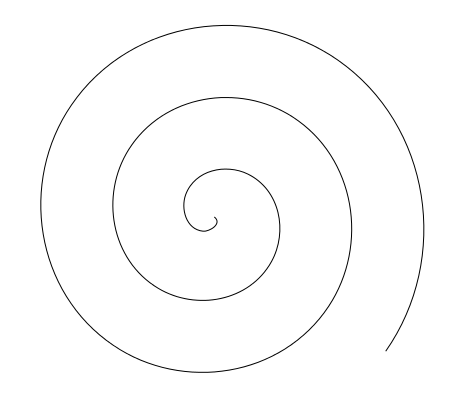
\includegraphics[width=\textwidth]{figures/pic01}
  \caption{Рисунок}
  \label{fig:fig01}
\end{figure}

В \cite{Pup09} указано, что...

Кстати, про картинки. Во-первых, для фигур следует использовать \texttt{[ht]}. Если и после этого картинки вставляются <<не по ГОСТ>>, т.е. слишком далеко от места ссылки,~--- значит у вас в РПЗ \textbf{слишком мало текста}! Хотя и ужасный параметр \texttt{!ht} у окружения \texttt{figure} тоже никто не отменял, только при его использовании документ получается страшный, как в ворде, поэтому просьба так не делать по возможности.

\section{Существующие подходы к созданию всячины}

Известны следующие подходы...

\begin{enumerate}
\item Перечисление с номерами.
\item Номера первого уровня. Да, ГОСТ требует именно так~--- сначала буквы, на втором уровне~--- цифры.
Чуть ниже будет вариант <<нормальной>> нумерации и советы по её изменению.
Да, мне так нравится: на первом уровне выравнивание элементов как у обычных абзацев. Проверим теперь вложенные списки.
\begin{enumerate}
\item Номера второго уровня.
\item Номера второго уровня. Проверяем на длииииной-предлиииииииииинной строке, что получается.... Сойдёт.
\end{enumerate}
\item По мнению Лукьяненко, человеческий мозг старается подвести любую проблему к выбору
  из трех вариантов.
\item Четвёртый (и последний) элемент списка.
\end{enumerate}

Теперь мы покажем, как изменить нумерацию на «нормальную», если вам этого захочется. Пара команд в начале документа поможет нам.

\renewcommand{\labelenumi}{\arabic{enumi})}
\renewcommand{\labelenumii}{\asbuk{enumii})}

\begin{enumerate}
\item Изменим нумерацию на более привычную...
\item ... нарушим этим гост.
\begin{enumerate}
\item Но, пожалуй, так лучше.
\end{enumerate}
\end{enumerate}

В заключение покажем произвольные маркеры в списках. Для них нужен пакет \textbf{enumerate}.
\begin{enumerate}[1.]
\item Маркер с арабской цифрой и с точкой.
\item Маркер с арабской цифрой и с точкой.
\begin{enumerate}[I.]
\item Римская цифра с точкой.
\item Римская цифра с точкой.
\end{enumerate}
\end{enumerate}

В отчётах могут быть и таблицы~--- см. табл.~\ref{tab:tabular} и~\ref{tab:longtable}.
Небольшая таблица делается при помощи \Code{tabular} внутри \Code{table} (последний
полностью аналогичен \Code{figure}, но добавляет другую подпись).

\begin{table}[ht]
  \caption{Пример короткой таблицы с длинным названием на много длинных-длинных строк}
  \begin{tabular}{|r|c|c|c|l|}
  \hline
  Тело      & $F$ & $V$  & $E$ & $F+V-E-2$ \\
  \hline
  Тетраэдр  & 4   & 4    & 6   & 0         \\
  Куб       & 6   & 8    & 12  & 0         \\
  Октаэдр   & 8   & 6    & 12  & 0         \\
  Додекаэдр & 20  & 12   & 30  & 0         \\
  Икосаэдр  & 12  & 20   & 30  & 0         \\
  \hline
  Эйлер     & 666 & 9000 & 42  & $+\infty$ \\
  \hline
  \end{tabular}
  \label{tab:tabular}
\end{table}

Для больших таблиц следует использовать пакет \Code{longtable}, позволяющий создавать
таблицы на несколько страниц по ГОСТ.

Для того, чтобы длинный текст разбивался на много строк в пределах одной ячейки, надо в
качестве ее формата задавать \texttt{p} и указывать явно ширину: в мм/дюймах
(\texttt{110mm}), относительно ширины страницы (\texttt{0.22\textbackslash textwidth})
и~т.п.

Можно также использовать уменьшенный шрифт~--- но, пожалуйста, тогда уж во \textbf{всей}
таблице сразу.

\begin{center}
  \begin{longtable}{|p{0.40\textwidth}|c|p{0.30\textwidth}|}
    \caption{Пример длинной таблицы с длинным названием на много длинных-длинных строк}
    \label{tab:longtable}
    \\ \hline
    Вид шума & Громкость, дБ & Комментарий \\
    \hline \endfirsthead
    \subcaption{Продолжение таблицы~\ref{tab:longtable}}
    \\ \hline \endhead
    \hline \subcaption{Продолжение на след. стр.}
    \endfoot
    \hline \endlastfoot
    Порог слышимости             & 0     &                                                \\
    \hline
    Шепот в тихой библиотеке     & 30    &                                                \\
    Обычный разговор             & 60-70 &                                                \\
    Звонок телефона              & 80    & \small{Конечно, это было до эпохи мобильников} \\
    Уличный шум                  & 85    & \small{(внутри машины)}                        \\
    Гудок поезда                 & 90    &                                                \\
    Шум электрички               & 95    &                                                \\
    \hline
    Порог здоровой нормы         & 90-95 & \small{Длительное пребывание на более
    громком шуме может привести к ухудшению слуха}                                        \\
    \hline
    Мотоцикл                     & 100   &                                                \\
    Power Mower                  & 107   & \small{(модель бензокосилки)}                  \\
    Бензопила                    & 110   & \small{(Doom в целом вреден для здоровья)}     \\
    Рок-концерт                  & 115   &                                                \\
    \hline
    Порог боли                   & 125   & \small{feel the pain}                          \\
    \hline
    Клепальный молоток           & 125   & \small{(автор сам не знает, что это)}          \\
    \hline
    Порог опасности              & 140   & \small{Даже кратковременное пребывание на
    шуме большего уровня может привести к необратимым последствиям}                       \\
    \hline
    Реактивный двигатель         & 140   &                                                \\
                                 & 180   & \small{Необратимое полное повреждение
                                 слуховых органов}                                        \\
    Самый громкий возможный звук & 194   & \small{Интересно, почему?..}                   \\
  \end{longtable}
\end{center}

%%% Local Variables:
%%% mode: latex
%%% TeX-master: "rpz"
%%% End:

\chapter{Конструкторский раздел}
\label{cha:design}

В данном разделе проектируется новая всячина.

\section{Архитектура всячины}

\paragraph{Проверка} параграфа. Вроде работает.
\paragraph{Вторая проверка} параграфа. Опять работает.

Вот.

\begin{itemize}
\item Это список с <<палочками>>.
\item Хотя он и не по ГОСТ, кажется.
\end{itemize}

\begin{enumerate}
\item Поэтому для списка, начинающегося с заглавной буквы, лучше список с цифрами.
\end{enumerate}

Формула \ref{F:F1} совершено бессмысленна.

%Кстати, при каких-то условиях <<удавалось>> получить двойный скобки вокруг номеров формул. Вопрос исследуется.

\begin{equation}
a= cb
\label{F:F1}
\end{equation}


Окружение \texttt{cases} опять работает (см. \ref{F:F2}), спасибо И. Короткову за исправления..


\begin{equation}
a= \begin{cases}
 3x + 5y + z, \mbox{если хорошо} \\
 7x - 2y + 4z, \mbox{если плохо}\\
 -6x + 3y + 2z, \mbox{если совсем плохо}
\end{cases}
\label{F:F2}
\end{equation}

\section{Подсистема всякой ерунды}

Культурная вставка dot-файлов через утилиту dot2tex (рис.~\ref{fig:fig02}).

\begin{figure}
  \centering
% [width=0.5\textwidth] --- регулировка ширины картинки
  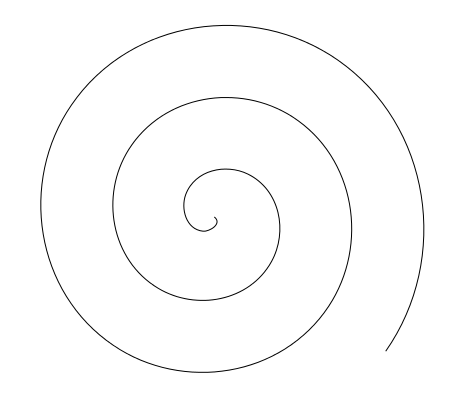
\includegraphics{figures/pic01}
  \caption{Рисунок}
  \label{fig:fig02}
\end{figure}


\subsection{Блок-схема всякой ерунды}

\subsubsection*{Кстати о заголовках}

У нас есть и \Code{subsubsection}. Только лучше её не нумеровать.

%%% Local Variables:
%%% mode: latex
%%% TeX-master: "rpz"
%%% End:

\chapter{Технологический раздел}
\label{cha:impl}

В данном разделе описано изготовление и требование всячины. Кстати,
в Latex нужно эскейпить подчёркивание (писать <<\verb|some\_function|>> для \Code{some\_function}).

\ifPDFTeX
Для вставки кода есть пакет \Code{listings}. К сожалению, пакет \Code{listings} всё ещё
работает криво при появлении в листинге русских букв и кодировке исходников utf-8.
В данном примере он (увы) на лету конвертируется в koi-8 в ходе сборки pdf.

Есть альтернатива \Code{listingsutf8}, однако она работает лишь с
\Code{\textbackslash{}lstinputlisting}, но не с окружением \Code{\textbackslash{}lstlisting}

Вот так можно вставлять псевдокод (питоноподобный язык определен в \Code{listings.inc.tex}):

\begin{lstlisting}[style=pseudocode,caption={Алгоритм оценки дипломных работ}]
def EvaluateDiplomas():
    for each student in Masters:
        student.Mark := 5
    for each student in Engineers:
        if Good(student):
            student.Mark := 5
        else:
            student.Mark := 4
\end{lstlisting}

Еще в шаблоне определен псевдоязык для BNF:

\begin{lstlisting}[style=grammar,basicstyle=\small,caption={Грамматика}]
  ifstmt -> "if" "(" expression ")" stmt |
            "if" "(" expression ")" stmt1 "else" stmt2
  number -> digit digit*
\end{lstlisting}

В листинге~\ref{lst:sample01} работают русские буквы. Сильная магия. Однако, работает
только во включаемых файлах, прямо в \TeX{} нельзя.

% Обратите внимание, что включается не ../src/..., а inc/src/...
% В Makefile есть соответствующее правило для inc/src/*,
% которое копирует исходные файлы из ../src и конвертирует из UTF-8 в KOI8-R.
% Кстати, поэтому использовать можно только русские буквы и ASCII,
% весь остальной UTF-8 вроде CJK и египетских иероглифов -- нельзя.

\lstinputlisting[language=C,caption=Пример (\Code{test.c}),label=lst:sample01]{listings/test.c}

\else

Для вставки кода есть пакет \texttt{minted}. Он хорош всем кроме: необходимости Python (есть во всех нормальных (нет, Windows, я не про тебя) ОС) и Pygments и того, что нормально работает лишь в \XeLaTeX.

Можно пользоваться расширенным BFN:

\begin{listing}[H]
\begin{ebnfcode}
 letter = "A" | "B" | "C" | "D" | "E" | "F" | "G"
       | "H" | "I" | "J" | "K" | "L" | "M" | "N"
       | "O" | "P" | "Q" | "R" | "S" | "T" | "U"
       | "V" | "W" | "X" | "Y" | "Z" ;
digit = "0" | "1" | "2" | "3" | "4" | "5" | "6" | "7" | "8" | "9" ;
symbol = "[" | "]" | "{" | "}" | "(" | ")" | "<" | ">"
       | "'" | '"' | "=" | "|" | "." | "," | ";" ;
character = letter | digit | symbol | "_" ;
 
identifier = letter , { letter | digit | "_" } ;
terminal = "'" , character , { character } , "'" 
         | '"' , character , { character } , '"' ;
 
lhs = identifier ;
rhs = identifier
     | terminal
     | "[" , rhs , "]"
     | "{" , rhs , "}"
     | "(" , rhs , ")"
     | rhs , "|" , rhs
     | rhs , "," , rhs ;
 
rule = lhs , "=" , rhs , ";" ;
grammar = { rule } ;
\end{ebnfcode}
\caption{EBNF определённый через EBNF}
\label{lst:ebnf}
\end{listing}

А вот в листинге \ref{lst:c} на языке C работают русские комменты. Спасибо Pygments и Minted за это.

\begin{listing}[H]
\cfile{inc/src/test.c}
\caption{Пример — test.c} 
\end{listing}
\label{lst:c}

\fi

% Для вставки реального кода лучше использовать \texttt{\textbackslash lstinputlisting} (который понимает
% UTF8) и стили \Code{realcode} либо \Code{simplecode} (в зависимости от размера куска).




Можно также использовать окружение \Code{verbatim}, если \Code{listings} чем-то не
устраивает. Только следует помнить, что табы в нём <<съедаются>>. Существует так же команда \Code{\textbackslash{}verbatiminput} для вставки файла.

\begin{verbatim}
a_b = a + b; // русский комментарий
if (a_b > 0)
    a_b = 0;
\end{verbatim}

%%% Local Variables:
%%% mode: latex
%%% TeX-master: "rpz"
%%% End:

\chapter{Экспериментальный раздел}
\label{cha:research}

В данном разделе проводятся вычислительные эксперименты.
А на рис.~\ref{fig:spire01} показана схема мыслительного процесса автора...

\begin{figure}
  \centering
  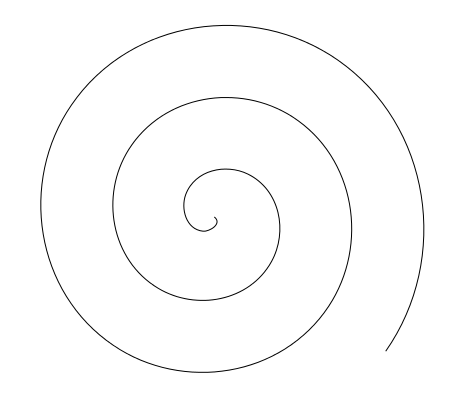
\includegraphics[width=\textwidth]{figures/pic01}
  \caption{Как страшно жить}
  \label{fig:spire01}
\end{figure}


%%% Local Variables:
%%% mode: latex
%%% TeX-master: "rpz"
%%% End:


\backmatter %% Здесь заканчивается нумерованная часть документа и начинаются ссылки и
            %% заключение

\Conclusion % заключение к отчёту

В ходе проделанной лабораторной работы, был изучен и
смоделирован бизнес-процесс оказания государственной
услуги <<Совет да любовь>>. В ходе этого моделирования,
удалось на практике ознакомится с методами анализа,
предоставляемыми Bizagi Process Modeler: описание
процесса в натации стандарта BPMN 2.0, временной анализ,
анализ затрат ресурсов, а также календарный анализ.

Во время проведения моделирования, было найдено одно
узкое место в моделируемом процессе -- обработка запроса
через ИЦ. После этого был проведен эксперимент в виде
сравнительного анализа "Что-Если", в котором мы
попытались проверить гипотезу, что процесс значительно
улучшится, если мы модернезируем ИЦ.

В результате этого анализа программа Bizagi Modeler
предоставила нам сравнительные таблицы, по которым мы пришли
к неоднозначным результатам: с одной стороны максимальное
время оказания услуги уменьшилось и стало допустимым с другой
среднее время выполнения увеличилось, за счет задержек
возникших на других этапах решения задачи.

Таким образом, требуется провести более комплексные экспеименты,
чтобы значительно повлиять на работу данного процесса.




%%% Local Variables:
%%% mode: latex
%%% TeX-master: "rpz"
%%% End:


% % Список литературы при помощи BibTeX
% Юзать так:
%
% pdflatex rpz
% bibtex rpz
% pdflatex rpz

\bibliographystyle{gost780u}
\bibliography{rpz}

%%% Local Variables: 
%%% mode: latex
%%% TeX-master: "rpz"
%%% End: 


\appendix   % Тут идут приложения

\chapter{Картинки}
\label{cha:appendix1}

\begin{figure}
\centering
\caption{Картинка в приложении. Страшная и ужасная.}
\end{figure}

%%% Local Variables: 
%%% mode: latex
%%% TeX-master: "rpz"
%%% End: 

\chapter{Еще картинки}
\label{cha:appendix2}

\begin{figure}
\centering
\caption{Еще одна картинка, ничем не лучше предыдущей. Но надо же как-то заполнить место.}
\end{figure}

%%% Local Variables: 
%%% mode: latex
%%% TeX-master: "rpz"
%%% End: 


\end{document}

%%% Local Variables:
%%% mode: latex
%%% TeX-master: t
%%% End:
